\bghdr{images/fond-mac}

%\begin{center}
%
\includegraphics{images/logo_Mac}
%\end{center}



\subsection{Configuration sous Mac OS X}

Sur Mac, branche toi au réseau, puis ouvre un navigateur et va sur \urllink{http://configuration} pour accéder à l'infoBR en ligne et la fin de la configuration.

%\subsubsection{Configuration IP}

%\flimage{images/mac_prefs_icone}{0.07}{l}
% \app{Préférences Réseau}, accessible depuis l'article de menu \menu{Préférences système} du menu \menu{Pomme}, permet de configurer la connexion au réseau. Par ailleurs, si au démarrage un assistant te propose de configurer ton réseau, refuse et utilise la procédure du BR. En effet, le réseau nécessite une configuration particulière à l'X, plus complexe que celle effectuée par cet assistant.
%
%
%\noindent
%  \begin{figure*}[h]
%    \begin{center}  
%     % \subfloat[Tiger]{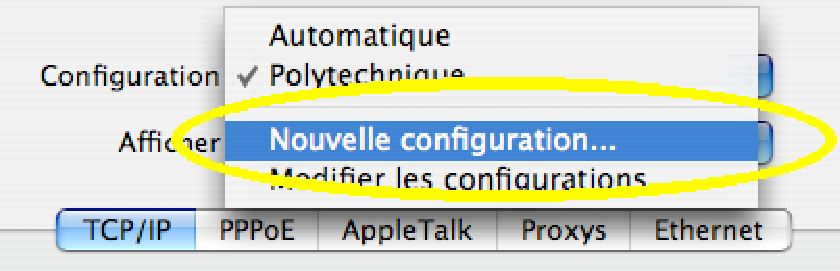
\includegraphics[width=0.47\textwidth]{images/mac_nouvelle_config} } 
%     % \hfill
%      \subfloat[Créer une nouvelle configuration réseau]{ 
%      \begin{minipage}{0.43 \textwidth}\begin{flushleft}
%      {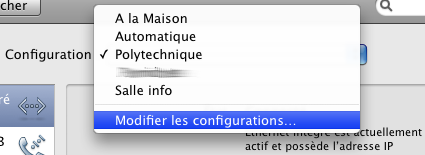
\includegraphics[width=0.96\textwidth]{images/mac_nouvelle_config_mountain_lion_1}}\\ \vspace*{2cm}
%      {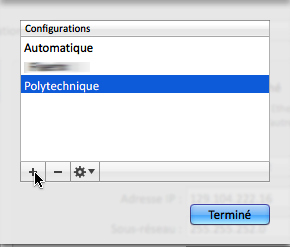
\includegraphics[width=0.96\textwidth]{images/mac_nouvelle_config_mountain_lion_2}} 
%        \end{flushleft}  \end{minipage}
%        }
%        \subfloat[Configuration de l'interface réseau \emph{Ethernet}, de l'adresse IP et du \emph{proxy}]{ 
%        \begin{minipage}{0.43 \textwidth}\begin{flushright}
%        {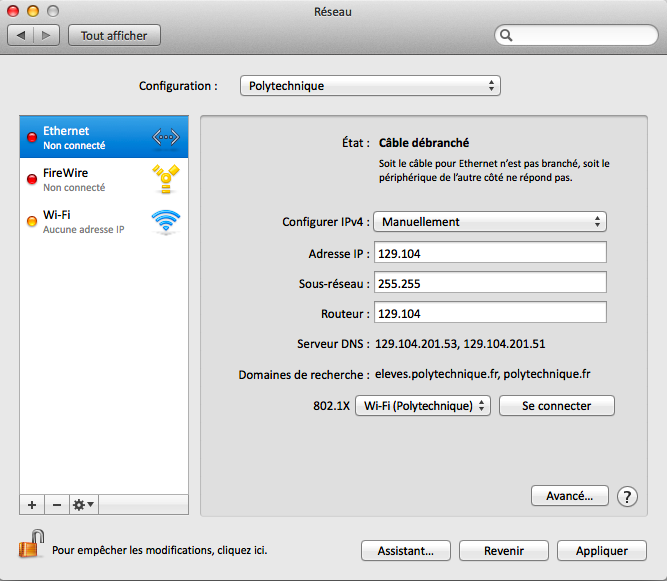
\includegraphics[width=0.96 \textwidth]{images/mac_config_ip_mountain_lion}} \\
%        {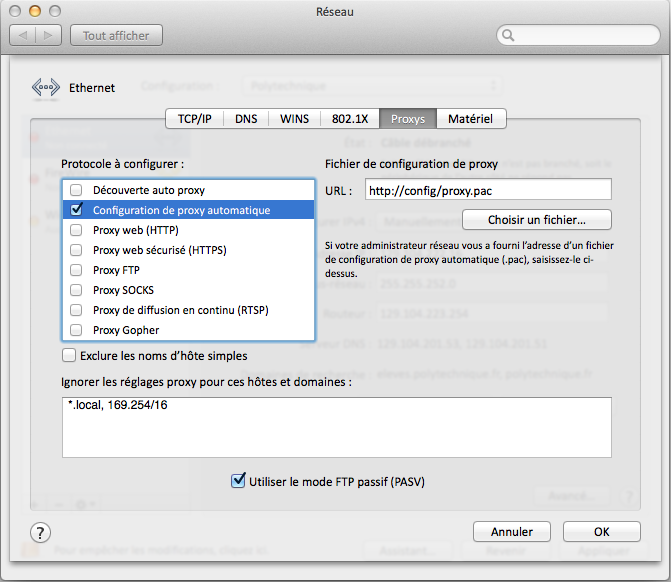
\includegraphics[width=0.96 \textwidth]{images/mac_config_proxy_mountain_lion}}
%        \end{flushright}
%        \end{minipage}
%            \label{config:mac:ip:mountain_lion}   }
%        \caption{Créer une nouvelle configuration réseau}
%
%    \end{center}
%  \end{figure*}
%
%%\pagebreak
%
%La gestion des configurations réseau de Mac OS X permet de créer plusieurs configurations et de passer en un clic de l'une  l'autre grâce au sous-menu \menu{Configuration Réseau} du menu \menu{Pomme}. Cela est très pratique pour les machines vouées à  être connectées à  plusieurs endroits successivement, typiquement les portables (voir la section \emph{Wi-Fi} page~\pageref{wifi} pour plus de précisions sur le \emph{Wi-Fi}). Commence donc par créer une nouvelle configuration réseau dans le menu déroulant \menu{Configuration}.
%\\
%\\
%Une fois la nouvelle configuration créée, il faut configurer l'interface réseau \emph{Ethernet}.
%
%
%\app{Mountain Lion \& Mavericks} : Dans la colonne de gauche, sélectionne \menu{Ethernet}.
%
%Choisis alors \menu{Configurer IPv4} : \menu{Manuellement}. Tu trouveras toutes les valeurs d'adresses IP nécessaires pour la configuration en page \pageref{calcul_ip} ou en te reportant aux captures d'écran~\ref{config:mac:ip:mountain_lion}. Remplis le champ \emph{Routeur} avec l'adresse de passerelle que tu as calculée. Si une partie d'adresse IP est blanche sur ces captures, c'est qu'elle t'est personnelle et que tu dois la calculer !
%
%
%  
%  
%
%%\imageref{images/mac_config_ip_leopard}{0.4}{Configuration IP (Leopard)}{!ht}{config:mac:ip:leopard}}
%\vspace{4mm}
%
%\textbf{Pour avoir accès à  Internet, il faut aussi configurer le \emph{serveur DNS} et le \emph{proxy}.}
%
%Configuration du \emph{serveur DNS} : clique sur le bouton \menu{Avancé...} puis va dans l'onglet \menu{DNS}. Ajoute les serveurs DNS 129.104.201.53 et 129.104.201.51 dans la colonne de gauche et les domaines de recherche \emph{eleves.polytechnique.fr} et \emph{polytechnique.fr} dans la colonne de droite.
%
%
%
%Configuration du \emph{proxy} : va dans l'onglet \menu{Proxys} et remplis l'URL comme dans la capture d'écran. N'oublie pas d'activer le mode passif pour les transferts en FTP, en cochant la case comme dans la capture.
%
%Sous Mac OS, le réglage du proxy se fait au niveau des préférences systèmes et n'a donc pas à être spécifié pour chaque navigateur. Tu peux donc sauter la partie \emph{Configuration de ton navigateur Web}.
%
%
%
%%\subsubsection{Configuration antivirus}
%
%%Bien qu'il soit important de maintenir ton système à  jour, un antivirus est pour l'instant tout à  fait superflu sur Mac,
%%puisqu'aucun virus fonctionnel n'a encore vu le jour. Attention cependant, n'ouvre pas des fichiers dont tu ne te sois pas assuré la provenance,
%%et essaie de te tenir au courant des actualités concernant les failles des applications que tu utilises.
%
%
%% \subsubsection{Autres logiciels utiles}
%
%%\flimage{images/mac_qrezix_icone}{0.07}{l} \app{qRezix} : en deux mots, c'est un programme développé par le BR pour faciliter la vie sur le réseau. Tu peux le récupérer via le lien qRezix sur \server{Frankiz} ou sur \urllink{http://br.frankiz.net/qrezix/mac/}. Pour plus de détails, voir le paragraphe consacré à  qRezix à  la page \pageref{qrezix}. \\
%
%%\app{Leopard} : le pare-feu se règle pour chaque application; tu n'auras qu'à  répondre \menu{Autoriser} lorsqu'il te demandera si tu veux \menu{Autoriser les connexions entrantes}.
%
%%\noindent  \app{Tiger} : Attention, si ton \emph{firewall} est activé, tu dois ouvrir les ports 5050, 5053 et 5055 en TCP. Pour cela va dans \app{Préférences Système}, dans le module \menu{Sécurité}, onglet \menu{Coupe-feu}. S'il est écrit \menu{Coupe-feu activé}, clique le bouton \menu{Nouveau} et remplis la boîte de dialogue comme sur la capture d'écran ci-dessous pour ouvrir les ports.
%
%%\imagepos{images/mac_firewall}{0.5}{Ouvrir les ports pour \app{qRezix} (Tiger)}{!ht}
%
%%\flimage{images/mac_conversation_icone}{0.1}{l}
%%\noindent\app{Colloquy}, un client IRC dans le même esprit qu'\app{iChat}. Il dispose d'une interface très simple ne nécessitant pas de connaître les commandes IRC. Tu peux te reporter à  la page \pageref{irc} pour plus d'infos sur l'IRC. \app{X-Chat Aqua} est un autre client IRC, plus riche en fonctionnalités, mais moins agréable à  utiliser. \\
%
%%\flimage{images/mac_netnewswire_icone}{0.1}{l}
%%\noindent\app{NetNewsWire} est la référence des clients RSS sur Mac, et est maintenant gratuit. Dans le même genre, on peut citer \app{Vienna}, un client RSS open source, dont le développement actif est prometteur. Les flux RSS permettent d'agréger dans un seul logiciel des informations en provenance de nombreux sites web, qui peuvent provenir de forums de discussions, de mises à  jour de logiciels, d'informations internationales\dots \\ \\
%
%% \label{mac-fink}
%% \flimage{images/mac_fink_icone}{0.07}{l} 
%%  \app{Fink} est la manière la plus simple d'installer sur Mac OS X nombre de logiciels issus du monde Unix (Linux par exemple). Grâce à  lui, tu pourras installer les mêmes logiciels que dans les salles informatiques. Par exemple, tu pourras installer Scilab sans trop de peine\dots La configuration nécessaire se trouve sur la page \urllink{https://br.binets.fr/Miroir\_Fink}.
%% 
%% \paragraph{}
%% \flimage{images/logo_Windows}{0.1}{l}
%%  \app{Windows et les Mac Intel} : Maintenant il est possible d'installer Windows grâce à  \app{Boot Camp}, livré avec \app{Leopard} et les version suivantes. Cela te permettra de profiter des quelques applications du monde PC qui valent le coup tout en gardant ton Mac. Tu peux également virtualiser Windows (utiliser Windows en utilisant en même temps Mac OS) grâce à  \app{VMware Fusion}, \app{VirtualBox} ou \app{Parallels Desktop}. Le  défaut de cette solution est que tu n'as pas d'accélération 3D, donc pour les jeux il te faudra redémarrer. Ces trois logiciels sont disponibles sur leurs sites \emph{web} respectifs. ÀA toi de choisir !

\clearpage